\documentclass[UTF8, a4paper, 11pt]{ctexart}

\usepackage[left=2.50cm, right=2.50cm, top=2.50cm, bottom=2.50cm]{geometry}
\usepackage{fontspec}
\usepackage{amsmath, amsfonts, amssymb, amsthm}
\usepackage{xcolor}
\usepackage{graphicx, float, subfigure}
\usepackage{url}
\usepackage{bm}
\usepackage{multirow}
\usepackage{booktabs}
\usepackage{epstopdf}
\usepackage{epsfig}
\usepackage{longtable, listings}
\usepackage{supertabular}
\usepackage{algorithm}
\usepackage{algorithmic}
\usepackage{changepage}

% \setmainfont{Times New Roman}

\renewcommand{\algorithmicrequire}{ \textbf{Input:}}     % use Input in the format of Algorithm
\renewcommand{\algorithmicensure}{ \textbf{Initialize:}} % use Initialize in the format of Algorithm
\renewcommand{\algorithmicreturn}{ \textbf{Output:}}     % use Output in the format of Algorithm
\renewcommand{\abstractname}{\textbf{\large{摘\quad 要}}} %更改摘要二字的样式

\theoremstyle{definition}

% \newtheorem{axiom}{\indent 公理}[chapter]
\newtheorem{theorem}{\indent 定理}[section]
\newtheorem{lemma}[theorem]{\indent 引理}
\newtheorem{proposition}[theorem]{\indent 命题}
\newtheorem{corollary}[theorem]{\indent 推论}
\newtheorem{definition}[theorem]{\indent 定义}
\newtheorem{example}{\indent 例}[section]
\newenvironment{solution}{\begin{proof}[\indent\bf 解]}{\end{proof}}
\renewcommand{\proofname}{\indent\bf 证明}

% \newtheorem{axiom}{\indent Axiom}[chapter]
% \newtheorem{theorem}{\indent Theorem}[section]
% \newtheorem{lemma}[theorem]{\indent Lemma}
% \newtheorem{proposition}[theorem]{\indent Proposition}
% \newtheorem{corollary}[theorem]{\indent Corollary}
% \newtheorem{definition}[theorem]{\indent Definition}
% \newtheorem{example}{\indent Example}[section]
% \newenvironment{solution}{\begin{proof}[\indent\bf Solution]}{\end{proof}}
% \renewcommand{\proofname}{\indent\bf Proof}

\newcommand{\xiaosi}{\fontsize{12pt}{\baselineskip}}     %\xiaosi代替设置12pt字号命令,不加\selectfont,行间距设置无效
\newcommand{\wuhao}{\fontsize{10.5pt}{10.5pt}\selectfont}
\newcommand{\degree}{^\circ}
\newcommand*{\dif}{\mathop{}\!\mathrm{d}}

\usepackage{fancyhdr} %设置全文页眉、页脚的格式
\pagestyle{fancy}
\lhead{}           %页眉左边设为空
\chead{}           %页眉中间
\rhead{}           %页眉右边
%\rhead{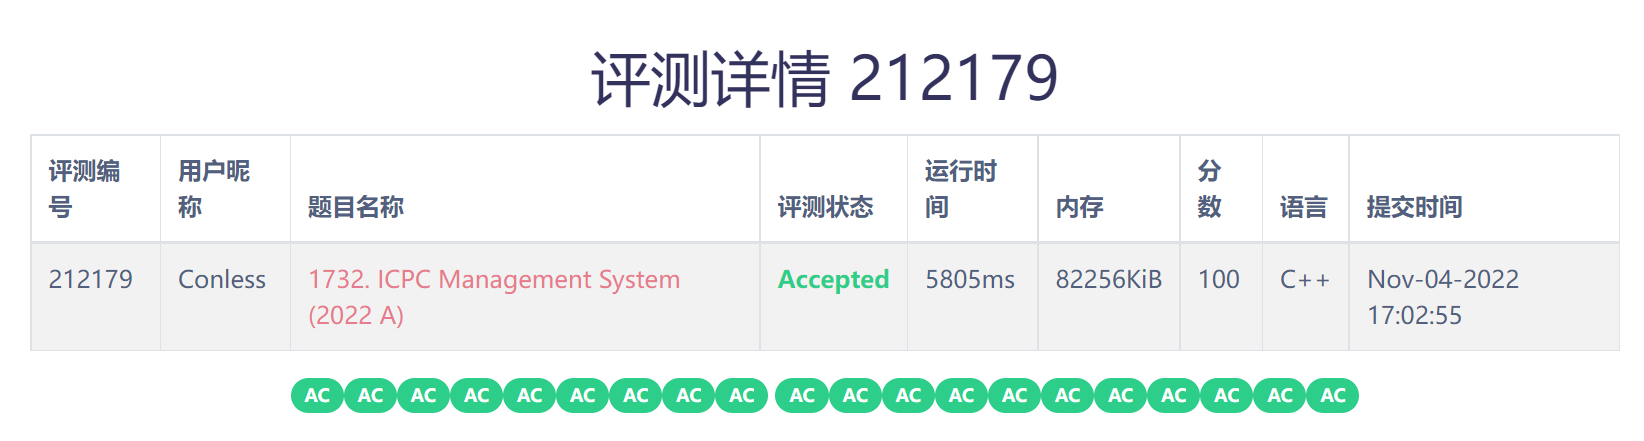
\includegraphics[width=1.2cm]{1.eps}}  %页眉右侧放置logo
\lfoot{}          %页脚左边
\cfoot{\thepage}  %页脚中间
\rfoot{}          %页脚右边

\lstset{
    basicstyle=\small\ttfamily,
    keywordstyle=\color{blue},
    commentstyle=\color{gray!50!black!50},
    backgroundcolor=\color{gray!5},
    stringstyle=\slshape\color{red},
    rulecolor=\color{gray!90},
    breaklines=true,
    frame=leftline,
    numbers=left,
	numberstyle=\footnotesize\itshape,
	firstnumber=1,
	stepnumber=1,
	numbersep=7pt,
}

\begin{document}

\thispagestyle{empty}

\begin{figure}[t]
    \centering
    \includegraphics[width=13cm]{/mnt/d/onedrive/resource/sjtu/logo/LogoChEnUD.png}
\end{figure}

\vspace*{\fill}
\begin{center}
    \Huge\textbf{ICPC Management System}\\
    \Huge\textbf{复杂度分析报告}
\end{center}
\vspace*{\fill}

\begin{table}[b]
    \centering
    \large
    \begin{tabular}{ll}
        \textbf{课程:}     & 程序设计 (A类) \\
        \textbf{课程编号:} & CS1953-01      \\
        \textbf{姓名:}     & 潘屹           \\
        \textbf{班级:}     & 电院2231       \\
        \textbf{时间:}     & 2022年11月     \\
        ~                                   \\
        ~                                   \\
        ~                                   \\
        ~                                   \\
        ~                                   \\
        ~                                   \\
    \end{tabular}
\end{table}

\newpage

\thispagestyle{empty}

\section{程序实现思路}

详见 https://github.com/Conless/HW2-ICPC-Management-System-2022/blob/master/intro.md 或者 https://www.conless.life/2022/11/354/.

\section{时间复杂度分析}

下面根据说明文档的要求, 对几个主要函数执行的时间复杂度进行分析.

\subsection{队伍比较}

这一部分在说明文档中不包含, 但实际上这直接决定了 set 操作的常数. 我最开始写的 compare 函数时间复杂度达到了 $O(m^2)$, 这是一个达到 $O (\sqrt{n})$ 级别的常数, 导致程序运行速度极慢, 后面换用新的方式比较 ac 时间, 就把这步的时间复杂度优化到了最坏 $O(m)$.

\begin{lstlisting}[language=C++]
bool TeamData::operator<(const TeamData &x) const {
    if (sub.ac_cnt != x.sub.ac_cnt)
        return sub.ac_cnt > x.sub.ac_cnt;
    if (penalty != x.penalty)
        return penalty < x.penalty;
    if (sub.ac_cnt) {   // Compare the ac time
        for (int i = sub.ac_cnt - 1; i >= 0; i--)
            if (ac_tim_sort[i] != x.ac_tim_sort[i])
                return ac_tim_sort[i] < x.ac_tim_sort[i];
    }
    return team_name < x.team_name;
}
\end{lstlisting}

\subsection{添加队伍}

对于添加队伍操作的实现在 src/ICPC.cc 中的 \texttt{void AddTeam(std::string)} 函数, 简要代码如下:

\begin{lstlisting}[language=C++]
void AddTeam(const std::string &team_name) {
    if (!started_flag) {                // Judge if the competition started
        if (!team_key[team_name]) {     // Judge if the team has been added
            std::cout << kAddTeamSuc << '\n';
            team_key[team_name] = team_cnt;
            team_list.push_back(TeamData(team_name, team_cnt));
            rank_list.insert(team_cnt);
            team_cnt++;
        } else {
            std::cout << kAddTeamDuplicated << '\n';
        }
    } else {
            std::cout << kAddTeamAfterStarted << '\n';
    }
    return;
}
\end{lstlisting}

主要的时间消耗发生在向记录排名的 set 中插入新的队伍编号, 根据红黑树的实现原理可以知道, 其平均与最坏时间复杂度均为 $O(\log n)$.

\subsection{提交题目}

在提交题目环节, 首先可以判断该题目是否处于不封榜下的通过 (Accepted) 状态, 如是, 需要对记录队伍排名的 set 进行更新, 否则只对队伍数据进行静态更新即可, 核心实现代码如下.

\begin{lstlisting}[language=C++]
void SubmitProblem(const std::string &problem_name, const std::string &team_name, const int submit_status, const int tim) {
    int problem_key = problem_name[0] - 'A';
    Submission new_sub(team_key[team_name], problem_key, submit_status, tim, submit_cnt++);
    if (!freeze_flag) {             // not frozen
        if (submit_status == kAC) { // update set and ac data
            rank_list.erase(new_sub.tid);
            team_list[new_sub.tid].submit(new_sub);
            rank_list.insert(new_sub.tid);
        } else {
            team_list[new_sub.tid].submit(new_sub);
        }
    } else {                        // add into another freeze data
        team_list[new_sub.tid].submitf(new_sub);
    }
}
\end{lstlisting}
这一步单次的最坏时间复杂度为在 set 的插入时产生的 $O(\log n)$.

\subsection{刷新榜单}

在刷新榜单的操作中, 只需要更新 vector 中队伍的排名即可, 并不需要对 set 进行任何操作, 只需要一遍遍历即可解决.

\begin{lstlisting}[language=C++]
void FlushBoard() {
    int rk_cnt = 0;
    for (auto it : rank_list) {
        team_list[it].rank = ++rk_cnt;
    }
    std::cout << kFlushSuc << '\n';
    return;
}
\end{lstlisting}

考虑到这里 set 寻值的操作是对地址进行 ++ 而不是挨个 find, 单次的 flush 操作只需要 $O(n)$ 即可完成.

\subsection{滚榜}

滚榜操作是整个实现过程中我认为最为复杂, 耗时最多的一步. 最开始我的实现思路为: 每一次从后往前找, 找到一个可以更新的队伍就刷新一遍榜单, 然后回到榜尾继续寻找, 直到完全没有可更新的队伍. 在这个过程中, 首先, 因为每一次要重新查榜, 所以单单遍历的最坏查询次数就可以达到 $\frac{1}{2}n(n-1)$, 对每支队伍每道题进行更新也有可能全部跑满, 即 $nm$, 即时间复杂度可以到达 $O(n^2)$, 这是一个巨大的消耗. 

但是, 我们可以注意到: 1. 除了 ac 以外的封榜后提交, 不会影响排名; 2. 查询过无封榜记录的队伍, 不需要再次进行查询. 这样一来, 就可以考虑预处理非 ac 提交, 滚榜只用实际操作 ac 提交; 并记录上一次查询的位置, 下一次扫就从该位置出发往上扫 (下面的一定不需要解冻).

由于完整代码过长, 这里给出伪代码的实现:


\begin{lstlisting}[language=C++]
void ScrollBoard() {
    /* Output the last scoreboard */
    for (auto it: rank_list)        // Unfreeze not-ac submission    
        if (team_list[it].frozen()) {
            for (int i = 0; i < problem_cnt; i++) {
                if (!team_list[it].aced_problem(i) && team_list[it].frozen(i)) {
                    team_list[it].unfreeze(i);
                }
            }
        }
    static std::vector<int> last_place;
    last_place.assign(team_cnt, 0);
    auto it_las = rank_list.end();
    do {                            // Unfreeze ac
        found_frz = 0;
        auto it = it_las;
        if (it == rank_list.begin())
            break;
        do {
            it_las = it;
            it--;
            if (team_list[*it].frozen()) {
                /* Update the data of *it */
            }
        } while (it != rank_list.begin());
    } while (found_frz);
    rk_cnt = 1;
    /* Output the new scoreboard */
    freeze_flag = 0;
}
\end{lstlisting}

其中, 对每支队伍每道题进行操作的最坏复杂度为 $O(nm)$, 对每一支 ac 队伍至多只需要进行一次 set 的删除插入, 时间复杂度为 $O(n\log n)$. 因此最坏时间复杂度为 $O(n\log n)$.

\subsection{查询}

查询队伍排名和队伍提交状态就相对简单, 可以在带有小常数的 $O(1)$ 时间内实现, 这里不做详细说明.

\section{测试结果}

本地测试 (WSL Ubuntu, 16GB RAM, AMD R7-5800H) 通过测试点 bigger, 使用 C++ clock() 记录的稳定在 1.1s 附近, Online Judge 上的通过总时间为 5.8s, 和 DarkSharpness 与 Polaris Dane 同学还有较大的差距.

\begin{figure}[H] 
    \centering
    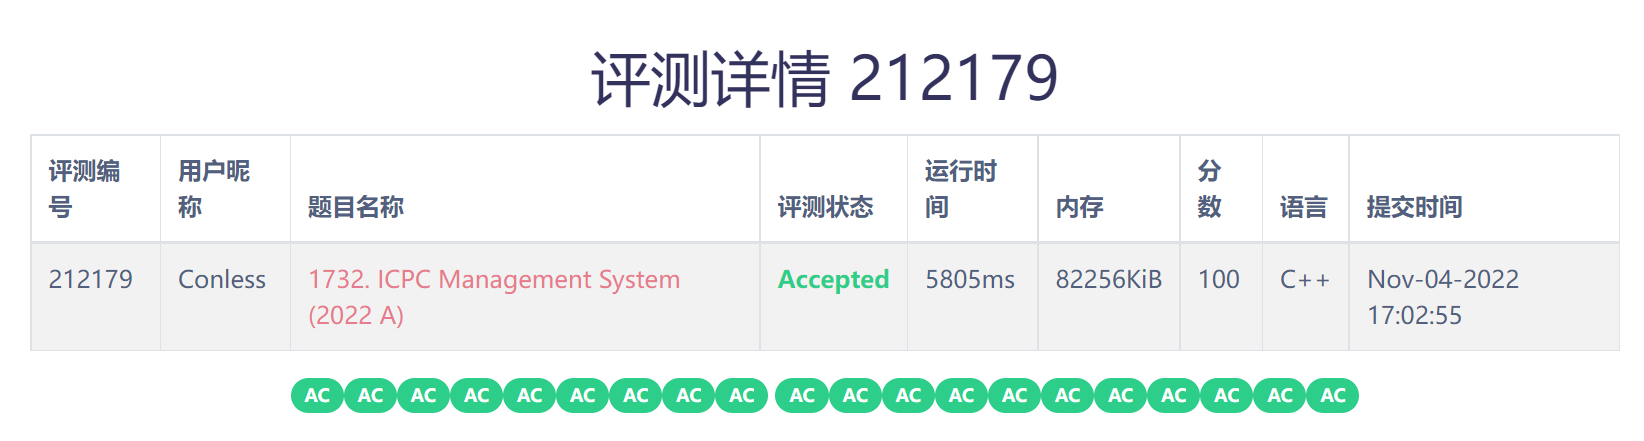
\includegraphics[width=0.4\textwidth]{1.png}
\end{figure}

可能是 set 没有进行空间优化造成每一次操作跑满 $\log n$, 以及 C++ STL 部分库模板的时间常数大于手写模板等多方面导致的, 但因为时间有限, 不再进行优化.

\end{document}